\documentclass{ximera}

\author{Jim Talamo}
\newcommand{\RR}{\mathbb R}
\renewcommand{\d}{\,d}
\newcommand{\dd}[2][]{\frac{d #1}{d #2}}
\renewcommand{\l}{\ell}
\newcommand{\ddx}{\frac{d}{dx}}
\newcommand{\dfn}{\textbf}
\newcommand{\eval}[1]{\bigg[ #1 \bigg]}


\title{Dig-In: Estimating Series}

\outcome{Define the remainder for a convergent series.}
\outcome{Estimate the value of a convergent series using the sequence of partial sums.}
\outcome{Explain the relationship between the remainder of a convergent series and the sequence of partial sums.}




\begin{document}
\begin{abstract}
    We learn how to estimate the value of a convergent series.
\end{abstract}
\maketitle

Given a series $\sum_{k=n_0}^{\infty} a_k$, we have discussed many ways to determine whether the series converges.  In the case when the series is geometric or telescoping and convergent, we can gives its value.  However, when the ratio test is used to determine that the series converges, it gives no information about the value to which the series converges.  Once we have established that the series converges, it's incredibly useful to be able to estimate its value, especially in the context of science or engineering.  

\section{Estimating Series}

\begin{model}
Consider the series $\sum_{k=1}^{\infty} \frac{1}{k^2}$.  

\begin{question}
Is this series geometric?
\begin{multipleChoice}
\choice{Yes}
\choice[correct]{No}
\end{multipleChoice}
\end{question}

\begin{question}
If we apply divergence test, note that $\lim_{n \to \infty} \frac{1}{n^2} = \answer{0}$, so the divergence test tells us \wordChoice{\choice{the series converges}\choice{the series diverges}\choice[correct]{nothing; it is inconclusive}}. 
\end{question}

\begin{question}
If we use ratio test, we find that $\lim_{n \to \infty} \left| \frac{a_{n+1}}{a_n} \right| = \lim_{n \to \infty} \left| \frac{n^2}{(n+1)^2} \right| = \answer{1}$, and thus the ratio test tells us \wordChoice{\choice{the series converges}\choice{the series diverges}\choice[correct]{nothing; it is inconclusive}}. 
\end{question}

None of the strategies we've seen thus far actually seem to help determine if this series converges.  There is a very creative  observation that we can make that will help by visualizing the series $\sum_{k=1}^{\infty} \frac{1}{k^2}$ as an ``area''.

Writing out a few terms in the sequence $\{a_n\}_{n=1}$ with $a_n = \frac{1}{n^2}$ gives the following list. 

\[
1, \, \frac{1}{4}, \, \frac{1}{9}, \, \frac{1}{16}, \, \dots 
\]

We now draw rectangles whose heights are the numbers in this list and whose widths are all $1$.


\begin{image}
\begin{tikzpicture}
	\begin{axis}[
            domain=0:6,xmin=-.1,xmax=4.5,ymin=-.1,ymax=1.2,
            width=4in,
            height=2in,
            xtick={1,2,...,4},
            ytick={1,.5,.333,.2},
            yticklabels={$a_1 = 1$,$a_2=1/4$,$a_3=1/9$,$a_4=1/16$},
            axis lines =middle, xlabel=$n$, ylabel=$a_n$,
            every axis y label/.style={at=(current axis.above origin),anchor=south},
            every axis x label/.style={at=(current axis.right of origin),anchor=west},
            axis on top,
          ]
          \addplot[color=penColor,fill=penColor,only marks,mark=*] coordinates{(1,1)};  %% closed hole
		\addplot [draw=penColor, fill = fillp] plot coordinates {(0,0) (1,0) (1, 1)(0,1) };   
		
          \addplot[color=penColor,fill=penColor,only marks,mark=*] coordinates{(2,1/2)};  %% closed hole
		\addplot [draw=penColor, fill = fillp] plot coordinates {(1,0) (2,0) (2, 1/2) (1,1/2) (1, 0)};          
          
	\addplot[color=penColor,fill=penColor,only marks,mark=*] coordinates{(3,1/3)};  %% closed hole
		\addplot [draw=penColor, fill = fillp] plot coordinates {(2,0) (3,0) (3, 1/3) (2,1/3) (2, 0)};          
          
          \addplot[color=penColor,fill=penColor,only marks,mark=*] coordinates{(4,1/5)};  %% closed hole
          	\addplot [draw=penColor, fill = fillp] plot coordinates {(3,0) (4,0) (4, 1/5) (3,1/5) (3, 0)};          

     
           %\addplot [draw=penColor,very thick,smooth, domain=.5:6] {1/x};
        \end{axis}
\end{tikzpicture}
\end{image}

Note that the area of the first rectangle is exactly $a_1 = 1$, the area of the second rectangle is exactly $a_2 = 1/4$, and so on.  If we continue drawing such rectangles, the total shaded area \textbf{exactly} represents to the sum $\sum_{k=1}^\infty\frac{1}{k^2}$.

A clever observation can be made by a plot of $1/x^2$ to our picture above.

\begin{image}
\begin{tikzpicture}
	\begin{axis}[
            domain=0:6,xmin=-.1,xmax=4.5,ymin=-.1,ymax=1.2,
            width=4in,
            height=2in,
            xtick={1,2,...,4},
            ytick={1,.5,.333,.2},
            yticklabels={$a_1 = 1$,$a_2=1/4$,$a_3=1/9$,$a_4=1/16$},
            axis lines =middle, xlabel={}, ylabel={},
            every axis y label/.style={at=(current axis.above origin),anchor=south},
            every axis x label/.style={at=(current axis.right of origin),anchor=west},
            axis on top,
          ]
          
                    \addplot[color=penColor,fill=penColor,only marks,mark=*] coordinates{(1,1)};  %% closed hole
		\addplot [draw=penColor, fill = fillp] plot coordinates {(0,0) (1,0) (1, 1)(0,1) };   
		
		
          \addplot[color=penColor,fill=penColor,only marks,mark=*] coordinates{(2,1/2)};  %% closed hole
		\addplot [draw=penColor, fill = fillp] plot coordinates {(1,0) (2,0) (2, 1/2) (1,1/2) (1, 0)};          
          
	\addplot[color=penColor,fill=penColor,only marks,mark=*] coordinates{(3,1/3)};  %% closed hole
		\addplot [draw=penColor, fill = fillp] plot coordinates {(2,0) (3,0) (3, 1/3) (2,1/3) (2, 0)};          
          
          \addplot[color=penColor,fill=penColor,only marks,mark=*] coordinates{(4,1/4)};  %% closed hole
          	\addplot [draw=penColor, fill = fillp] plot coordinates {(3,0) (4,0) (4, 1/4) (3,1/4) (3, 0)};          

           \addplot [draw=penColor,very thick,smooth, domain=.5:6] {1/x};
           
        \end{axis}
\end{tikzpicture}
\end{image}

Note that we have a slight annoyance if we consider $\int_{0}^{\infty} \frac{1}{x^2} \d x$ since $\frac{1}{x^2}$ has a vertical asymptote at $x=0$.  This is easily avoided if we instead consider $\frac{1}{x^2}$ on the interval $[1,\infty)$.  This requires that we consider the rectangles on that interval too.  We update our picture.


\begin{image}
\begin{tikzpicture}
	\begin{axis}[
            domain=0:6,xmin=-.1,xmax=4.5,ymin=-.1,ymax=1.2,
            width=4in,
            height=2in,
            xtick={1,2,...,4},
            ytick={1,.5,.333,.2},
            yticklabels={$a_1 = 1$,$a_2=1/4$,$a_3=1/9$,$a_4=1/16$},
            axis lines =middle, xlabel={}, ylabel={},
            every axis y label/.style={at=(current axis.above origin),anchor=south},
            every axis x label/.style={at=(current axis.right of origin),anchor=west},
            axis on top,
          ]

		
		
          \addplot[color=penColor,fill=penColor,only marks,mark=*] coordinates{(2,1/2)};  %% closed hole
		\addplot [draw=penColor, fill = fillp] plot coordinates {(1,0) (2,0) (2, 1/2) (1,1/2) (1, 0)};          
          
	\addplot[color=penColor,fill=penColor,only marks,mark=*] coordinates{(3,1/3)};  %% closed hole
		\addplot [draw=penColor, fill = fillp] plot coordinates {(2,0) (3,0) (3, 1/3) (2,1/3) (2, 0)};          
          
          \addplot[color=penColor,fill=penColor,only marks,mark=*] coordinates{(4,1/4)};  %% closed hole
          	\addplot [draw=penColor, fill = fillp] plot coordinates {(3,0) (4,0) (4, 1/4) (3,1/4) (3, 0)};          

           \addplot [draw=penColor,very thick,smooth, domain=.5:6] {1/x};
           
        \end{axis}
\end{tikzpicture}
\end{image}
Notice that the sum of the areas of the rectangles now is the series \wordChoice{\choice{$\sum_{k=0}^{\infty} \frac{1}{k^2}$}\choice{$\sum_{k=1}^{\infty} \frac{1}{k^2}$}\choice[correct]{$\sum_{k=2}^{\infty} \frac{1}{k^2}$}}.

This is not an issue, because we know

\begin{quote}
The value of the lower index of summation does not affect whether an infinite series converges or diverges.
\end{quote}

That is, if we can show $\sum_{k=2}^{\infty} \frac{1}{k^2}$ converges, then $\sum_{k=1}^{\infty} \frac{1}{k^2}$ must also converge.  Now to determine whether $\sum_{k=2}^{\infty} \frac{1}{k^2}$ converges, let $s_n = \sum_{k=2}^n \frac{1}{k^2}$.  Try to interpret $s_n$ in terms of the picture.  What area does it represent?

Now, we must determine if $\lim_{n \to \infty} s_n$ exists.  Since $s_n$ is \wordChoice{\choice[correct]{increasing}\choice{decreasing}}, the only way this limit cannot exist is if the terms $s_n$ become arbitrarily large.

Note that for any $n \geq 2$, we can observe from the picture that the area of the rectangles from $x=2$ to $x=n$ is \wordChoice{\choice[correct]{less than}\choice{equal to}\choice{greater than}} the ``area'' under the curve for $x \geq 1$.  This is represented by the inequality

\[
s_n = \sum_{k=1}^n\frac{1}{k^2} \leq
\int_1^\infty \frac{1}{x^2} \d x.
\]
We can calculate the value of this improper integral to find

\[
\int_1^\infty \frac{1}{x^2} \d x = \answer{1}.
\]

Thus, the terms in the sequence $\{s_n\}$ cannot become arbitrarily large, so $\lim_{n \to \infty} s_n$ must exist and from the picture, it must be less than the value of the improper integral.  Thus,$\sum_{k=1}^{\infty} \frac{1}{k^2}$  converges, but we do not yet know its value.  However, since 


\[\sum_{k=1}^{\infty} \frac{1}{k^2} = 1 +  \sum_{k=2}^{\infty} \frac{1}{k^2} \leq 1 + 1 =2, \] 

we have  $\sum_{k=1}^{\infty} \frac{1}{k^2} \leq 2$.

Suppose now that we want to \emph{approximate} the infinite series $\sum_{k=1}^{\infty} \frac{1}{k^2}$ better.  We can note that the sequence of partial sums, $\{s_n\}_{n=1}$ defined by $s_n = \sum_{k=1}^{n} \frac{1}{k^2}$, is an \wordChoice{\choice[correct]{increasing}\choice{decreasing}} sequence, so as $n$ increases, we expect that the \emph{finite} sum $\sum_{k=1}^{n} \frac{1}{k^2}$ should become \wordChoice{\choice[correct]{closer to}\choice{farther from}} the infinite series $\sum_{k=1}^{\infty} \frac{1}{k^2}$.  Indeed, by using technology (such as Wolfram Alpha, MatLab, Maple, etc) we can compute the following to $4$ decimal places.

\begin{itemize}
\item $s_4 =  \sum_{k=1}^{4} \frac{1}{k^2} = \frac{1}{1^2}+  \frac{1}{2^2}+ \frac{1}{3^2}+ \frac{1}{4^2} = \answer[tolerance=.0001]{1.4236}$.
\item $s_{10} =  \sum_{k=1}^{10} \frac{1}{k^2} = \frac{1}{1^2}+  \frac{1}{2^2}+ \ldots + \frac{1}{10^2} = \answer[tolerance=.0001]{1.5498}$.
\item $s_{100} = \sum_{k=1}^{100} \frac{1}{k^2} = \answer[tolerance=.0001]{1.6350}$.
\item $s_{1000} = \sum_{k=1}^{n} \frac{1}{k^2} = \answer[tolerance=.0001]{1.6439}$.
\end{itemize}


\end{model}

We can now ask an important question: just how close to the actual value of the infinite series $\sum_{k=1}^{\infty} \frac{1}{k^2}$ are these estimates?  Before tackling this question, we summarize some ideas presented in this example.
  
\begin{quote}
For a \emph{convergent} infinite series, we can truncate the series and use the finite sum $\sum_{k=1}^{n} a_k$ to estimate the value of $\sum_{k=1}^{\infty} a_k$.
\end{quote}

We now introduce an important new quantity, called the \emph{remainder}. 

\begin{definition}
Let $ \sum_{k=1}^\infty a_k$ be a convergent series.  The remainder term $r_n$ is defined by
\[
r_n := \sum \limits_{k=n+1}^{\infty} a_k.
\]

The remainder $r_n$ is the error made when using $s_n = \sum_{k=1}^n a_k$ to approximate the value of the infinite series $ \sum_{k=1}^\infty a_k$.
\end{definition}

Notice that $r_n$ is also an infinite series, and that its index starts at $n+1$.  The reason for writing the starting index in this way is so that we can think of splitting up the sum $S = \sum \limits_{k=1}^\infty a_k$ into our estimate, $s_n$, and our remainder $r_n$.

\begin{image}
  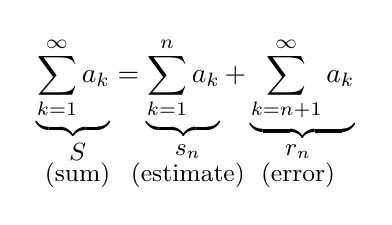
\begin{tikzpicture}
        \node at (0,0) {
           $\underbrace{\sum \limits_{k=1}^\infty a_k}  = \underbrace{\sum \limits_{k=1}^n a_k} + \underbrace{\sum \limits_{k=n+1}^\infty a_k} $ 
           };
        \node at (-0.1,-.8) {\small{$s_n$}};
        \node at (-0.1,-1.1){\small{(estimate)}};
        \node at (1.3, -.8) {\small{$r_n$}};
        \node at (1.3,-1.1) {\small{(error)}};
        \node at (-1.5, -0.8) {\small{$S$}};
        \node at (-1.5, -1.1) {\small{(sum)}};
      \end{tikzpicture}
  \end{image} 

\begin{remark}
Finding the exact value of the series $\sum_{k=1}^{\infty} \frac{1}{k^2}$ is not easy!  In fact, this problem was first posed by the Italian mathematician Pietro Mengoli in 1650 and became known as the Basel problem. The problem remained unsolved for nearly 100 years. In 1734, the famous mathematician Leonard Euler finally correctly found that $\sum_{k=1}^{\infty} \frac{1}{k^2} = \frac{\pi^2}{6}$ .  
\end{remark}

Overall, there are two main types of questions we would like to answer about remainders.
\begin{enumerate}
    \item If we use a specified number of terms, that is, if we pick $N$ and use $\sum_{k=1}^N a_k$ to approximate $\sum_{k=1}^{\infty} a_k$, how bad could the resulting error be?
    \item How many terms of a series (what is the value of $N$) should we use to obtain the estimate to a desired precision?
\end{enumerate}

While they are worded similarly, the two questions describe different situations in which we might find ourselves.  In the first, we want to add a specified number of terms - perhaps due to limitations in technology, memory space, or time.  Remember - estimating the error is a practical matter!  In the second, we want to achieve a specified precision, or make the error smaller than some specified threshold.  Again, in any practical circumstance, the threshold will likely be decided by safety specifications, sensitivity of instrumentation, or a required number of significant figures. 

We finish this section with an example that motivates a plausible theorem.


\begin{example}
Suppose that $\{a_n\}_{n=1}$ is a sequence and it is known that $\sum_{k=1}^{n} a_k = \frac{2n}{n+1}$.  
\begin{enumerate}
    \item Explain why the series $\sum_{k=1}^{\infty} a_k$ converges, and why its convergence is significant towards finding the remainder.
    \item Find an explicit formula for $r_n$.
    \item Find an integer $N$ so $\sum_{k=1}^{N} a_k$ is within $.01$ of the exact value of $\sum_{k=1}^{\infty} a_k$.
\end{enumerate} 

\begin{explanation}
\begin{enumerate}
\item Note that we are actually given that $s_n = \frac{2n}{n+1}$.  Since $\lim_{n \to \infty} s_n = \answer{2}$, we have that $\sum_{k=1}^{\infty} a_k$ \wordChoice{\choice{diverges}\choice[correct]{converges to $2$}} .

Since the series \wordChoice{\choice{diverges}\choice[correct]{converges}}, it makes sense to talk about the remainder $r_n$ for any $n \geq 1$, since $r_n$ will be a finite number for each $n$.  

\item Notice that the relationship $\sum_{k=1}^{\infty} a_k = s_n+r_n$ allows us to find an explicit formula for $r_n$.
\begin{align*}
\sum_{k=1}^{\infty} a_k &= s_n+r_n \\
2 &= \frac{2n}{n+1}+r_n \\
r_n &= 2-\frac{2n}{\answer[given]{n+1}}
\end{align*}


\item This question is really asking how many terms we need in a finite sum to ensure that the computed value will be accurate to $.01$ of the exact value of the infinite series.  Since $r_N$ will measure the error resulting from approximating the infinite series by $s_N$, we find $N$ by setting $\vert r_N \vert \leq .01$.  We can choose any value of $N$ which will satisfy this property.  Let's choose to find the smallest such value of $N$, since we have a nice procedure for doing so.

\begin{align*}
2-\frac{2N}{N+1} &\leq \frac{1}{100} \\
200-\frac{200N}{N+1} & \leq 1 \\
\frac{200N}{N+1} & \geq 199 \\
200N & \geq 199N+199 \\
N \geq \answer[given]{199}
\end{align*}

We thus know that $s_{199}$ can be used to approximate the value of $\sum_{k=1}^{\infty} a_k$ to within $.01$ of its exact value.  Notice that any value of $N$ which is greater than $199$ will also satisfy this property!  To be consistent, we will often ask specifically for the smallest possible value of $N$.
\end{enumerate}
\end{explanation}

\end{example}

Another thing to notice about the previous example: since we found a formula for $r_n = 2 - \frac{2n}{n+1}$, it's easy to see that $\lim \limits_{n \to \infty} r_n = 0$. In other words, if we increase the value of $n$, we decrease the error.  Said another way, the more terms we use when approximating a convergent series, the smaller our error should be in general.  This is part of a more general statement about the relationship between converging series and their remainders.

\begin{theorem}[Remainders and Convergence]\index{remainders and convergence}
Consider the series $\sum_{k=n_0}^{\infty} a_k$ and for every $n \geq n_0$, define $r_n = \sum_{k=n+1}^{\infty} a_k$.  If $\sum \limits_{k=1}^\infty a_k$ converges, then $\lim \limits_{n \to \infty} r_n = 0$.   
\end{theorem}

This theorem hopefully makes sense: if we think of 
\[
r_n = \sum \limits_{k=1}^\infty a_k - s_n,
\]
and we take the limit as $n$ goes to infinity on both sides, we know that $\lim \limits_{n \to \infty} s_n = \sum \limits_{k=1}^\infty a_k$ by the meaning of $s_n$.  The left hand side, or $r_n$, thus can be made as small as we wish.



\end{document}